\documentclass[conference,letterpaper,10pt]{IEEEtran}
\IEEEoverridecommandlockouts
\usepackage[T1]{fontenc}
\usepackage[utf8]{inputenc}
\usepackage{amsmath,amssymb,graphicx,booktabs,siunitx,balance}
\usepackage[hidelinks]{hyperref}
\sisetup{detect-weight=true,detect-family=true}
\newcommand{\nis}{\ensuremath{\mathrm{NIS}}}

% ── CAMERA-READY SWITCH ───────────────────────────────────────────────────────────────────────────
% \camerareadytrue reveals the funding acknowledgement below. It MUST stay false for the anonymous
% submission: the grants name the Junta de Extremadura and a POCTEP regional programme, which
% identifies the institution to any reviewer in the field as surely as a letterhead would. Reviewers
% do read acknowledgements, and this is the most common way a double-blind submission de-anonymises
% itself. Flip it for the final version only.
\newif\ifcameraready
\camerareadyfalse

% ── PAGE BUDGET: WHAT THE CAMERA-READY VERSION WILL COST US ───────────────────────────────────────
% The limit is 8 pages. This blind draft is 7 and its text stops 301 pt up the right column of p7,
% so roughly 1.2 pages are still free. But the final version is LONGER than what we can see here,
% and the growth lands at the two ends of the paper:
%   - the author block replaces two anonymous lines with names, two affiliations and an e-mail line;
%   - the funding paragraph above appears (7 lines), pushing the bibliography down by its own height.
% MEASURED, not estimated: a test build with \camerareadytrue and a representative 5-author, two-
% affiliation block moved the end of the paper down by 37 pt (~3.5 lines) and stayed on 7 pages.
% So reserve 37 pt at the end of p8 and the usable budget for NEW material is ~1583 pt of single
% column ≈ 144 lines ≈ 2.4 columns. Re-measure after adding anything: a figure that reflows a float
% can cost a page on its own, and the 29 references still missing a venue/year will each grow a line.

\begin{document}

\title{Calibrated Uncertainty for Active Room-Layout Estimation}

\author{\IEEEauthorblockN{Anonymous}\IEEEauthorblockA{Anonymous Institution}}

\maketitle

\begin{abstract}
A robot that estimates the layout of a room usually reports geometry and little else. Downstream
consumers---planners, scene graphs, other agents---must then decide how far to trust it, with nothing
to go on. We present an online room-layout estimator whose reported uncertainty is calibrated against
ground truth, and which uses that uncertainty as a decision variable: it gates which corners are
published, and it is what the robot acts to reduce. Parameters and structure (how many walls there
are) are inferred by minimising a variational free energy; viewpoint selection minimises the
corresponding expected free energy, whose epistemic term reduces to expected information gain under
the Gaussian model. The shared currency is what lets the data fit, the model complexity and the value
of the next observation be compared at all, and the calibrated uncertainty is what the robot acts on. On 594 annotated
floor plans the estimator reaches \num{0.983} mean IoU, and---our central result---a corner it
declares publishable has a median true error of \SI{2.0}{\centi\meter} and lies within its declared
\SI{6}{\centi\meter} in \SI{86}{\percent} of cases, against \SI{3.6}{\centi\meter} and
\SI{64}{\percent} for corners it withholds. Holding the system to that standard proved diagnostic:
it exposed three distinct precision defects in three different modules, all instances of uncertainty
that averages away past an error that does not, one of them in a module the instrument was not
measuring. A single global precision is insufficient for this problem: the part of the error that does not
average is several times larger than the part that does, it depends on the viewpoint rather than on
the map, and the precision declared for it is smaller than it---so a constant calibrated under one
condition need not remain calibrated under another, and precision should be inferred rather than
tuned.
\end{abstract}

\section{Introduction}

Room-layout estimation is mature enough that accuracy alone no longer separates methods. What
separates them for a robot is whether the estimate can be \emph{acted on}: whether a planner can tell
a wall that is known to a centimetre from one that is a guess, whether a scene graph should commit a
corner to shared memory, whether the robot should look again before deciding. All of these are
questions about uncertainty, and almost no layout system answers them with a number that has been
checked.

\begin{figure}[t]
\centering
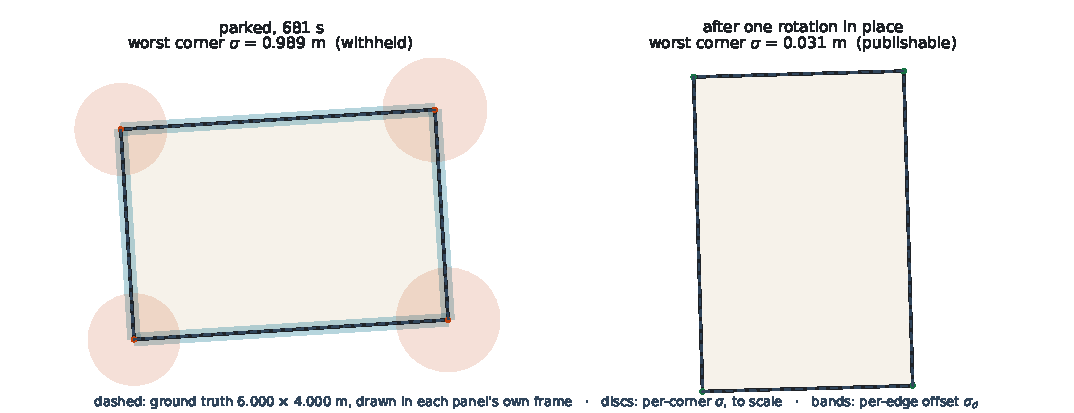
\includegraphics[width=\columnwidth]{fig/teaser}
\caption{\textbf{The estimate is right before it is confident, and says so.} One closed-loop run; the
same room in both panels, same scale, long axis horizontal. Pale band: ground truth, each dimension
carrying its measured value and signed error. Discs: per-corner $\sigma$, to scale. \emph{Left}, parked for
\SI{665}{\second}: the geometry is already within \SI{13}{\milli\meter} of truth, yet every corner
declares almost a metre of uncertainty and the layout is withheld. \emph{Right}, the first publishable
frame, after a turn in place: the geometry moves by at most \SI{6}{\milli\meter}, and stays within
\SI{19}{\milli\meter} of truth, while corner $\sigma$ falls by a factor of \num{21}. The estimator does not earn
precision by waiting, and does not claim any.}
\label{fig:teaser}
\end{figure}

This is not an oversight of presentation. An uncertainty that is never validated tends to be wrong, and
wrong in a way that is invisible: an estimator that overstates its error is merely timid, while one
that understates it is confidently incorrect, and neither shows up in a mean IoU. We found both
failure modes in our own system, and we found them only because something downstream was made to
depend on the number being right.

Our estimator maintains a room as a cyclic polygon of wall landmarks in Hesse normal form, inferred
jointly with the robot pose over a sliding window. Three decisions that are usually taken by three
separate mechanisms are here taken by one. \emph{What the walls are} is variational inference over
their parameters. \emph{How many walls there are} is Bayesian model comparison: a structural change
is adopted when it pays for its own description length, priced in nats on the same scale as the data
fit, rather than by a merge threshold. \emph{Where to look next} is the epistemic term of the expected
free energy, so the robot moves to reduce the uncertainty that is currently blocking it from
committing to a layout. Because all three are denominated in the same currency, every precision in
the model carries weight: get one wrong and the comparisons it feeds are priced in a corrupt unit.
That is the property we exploit.

\emph{Contributions.}
\begin{enumerate}
  \item An online layout estimator whose per-corner and per-edge uncertainty is \emph{validated
  against ground truth} on 594 annotated floor plans, and is \emph{actionable}: it gates publication
  and is the quantity the explorer acts to reduce (\S\ref{sec:exp}). We also report where that
  buys nothing: against a heuristic explorer on the same corpus the difference is null, and we say
  why.
  \item A propagation from returns to corner covariance that separates the error that averages down
  with more observation from the error that does not, and a measurement of both terms on real sensor
  data (\S\ref{sec:real}).
  \item Evidence that a single global precision is insufficient for this problem: the non-averaging
  part of the error is several times larger than the averaging part, it is viewpoint-dependent rather
  than a property of the map, and the declared pose precision does not cover it---measured in
  simulation and reproduced on a physical robot (\S\ref{sec:notconstant}).
  \item Three precision defects found by calibration, including one localised in a module the
  statistic was not measuring---offered as evidence that a free-energy formulation is useful
  diagnostically, not only descriptively.
\end{enumerate}

\section{Related Work}

\emph{Floor-plan reconstruction from complete scans.} A large family of methods recovers a floor
plan from an accumulated point cloud or density image, from the early unified
formulation~\cite{liu2018floornet} and its shortest-path successor~\cite{chenfloorsp} through
attention and query-based architectures~\cite{chen2022heat,yue2023roomformer}, room-wise implicit and
slicing representations~\cite{xufrinet,su2023slibonet}, room-aware
transformers~\cite{liu2024polyroom}, continuity-aware edges~\cite{liu2025cage}, guided set
diffusion~\cite{chen2023polydiffuse}, autoregressive polygon
sequences~\cite{phung2026raster2seq}, and segmentation-guided
fusion~\cite{ye2025floorsam}. They are evaluated by corner and room F1 on a finished scan. Two
properties distinguish them from our setting: they are offline, so no decision is taken while the
estimate is still uncertain; and the number of corners is chosen by a search with hand-set costs
rather than by a likelihood, so there is no quantity in which structure and data fit are commensurate.

\emph{Panoramic room layout.} Single- and multi-view layout estimation recovers room shape from
$360^\circ$ imagery~\cite{hu2021mvlayoutnet,su2022gprnet,wangpsmnet}, with self-training and
multi-view consistency removing the need for per-scene labels~\cite{solarte2022mlc,
solarte2024raycasting}, and related work registering panoramas or verifying their
alignment~\cite{hutchcroftcovispose,lambertsalve}. These produce a layout per view rather than a
belief a robot accumulates, and report no per-corner uncertainty a consumer could gate on. Unbounded
and general (non-Manhattan) variants relax the shape prior~\cite{howardjenkins2019unconstrained,
fayyazsanaviu2rle,bieri2025houselayout3d}. \emph{Sequential} floor-plan estimation from a moving
camera~\cite{solarte2022dfpe} is the closest in spirit to ours: it, too, must decide room
membership and shape while the scene is still incomplete. Autoregressive scene
description~\cite{avetisyan2024scenescript} likewise produces structure from a walkthrough, as
language rather than as a belief with a covariance.

\emph{Exploration that predicts structure.} A complementary line predicts unobserved layout to
drive exploration---room shape from partial observation~\cite{luperto2020exploration}, walls beyond
the frontier learned from floor plans~\cite{ericson2024floorist}, information gain from global map
predictions~\cite{ho2025mapex}, and generative layout prediction for
planning~\cite{wang2025cogniplan}---together with the question of when a map is
finished~\cite{luperto2024mapcompleteness}. These share our premise that a layout belief should
inform where to go next; the predicted structure is used to \emph{score} viewpoints rather than to be
published with an uncertainty a downstream consumer must trust.

\emph{Active SLAM.} Surveys of the field~\cite{ahmed2023aslamreview,placed2023survey} formalise
viewpoint selection by information-theoretic utility, and the question of whether the usual
uncertainty criteria are the right ones has itself been raised~\cite{placed2022enough}. Our selection
rule is the epistemic term of an expected free energy, which coincides with information gain under a
Gaussian model; the contribution here is not the rule but that the precision it consumes has been
verified, so the gain it predicts is a gain that exists.

\emph{Uncertainty and calibration.} Uncertainty estimation is well studied in dense depth
prediction, where predicted confidence can be compared against realised error~\cite{poggiuncertainty},
and in photogrammetric modelling~\cite{jarzabek2022uncertainty,liu2024point2building}. To our
knowledge no online room-layout estimator reports a per-corner covariance that has been validated
against layout ground truth, which is the gap this paper addresses. Our position is deliberately
parametric: we keep a covariance rather than a coverage set, because a joint estimator and a
downstream consumer both need one, and we check it.

\emph{What the two literatures leave open.} Layout methods are evaluated on geometric
accuracy; none of them calibrates a \emph{per-corner} uncertainty against the error it actually makes,
so a consumer is given a shape and no basis for trusting any part of it more than another. Active
SLAM and next-best-view methods do consume a covariance, but they inherit whichever one the estimator
produces and rarely ask whether that covariance predicts the realised error --- an acquisition policy
driven by an over-confident covariance will stop moving precisely where it should not. The two gaps
are the same gap seen from opposite sides. Our contribution joins them: we calibrate the layout's
uncertainty against ground truth, and then use the calibrated quantity for both jobs it is fit for ---
as the criterion that decides which geometry may be published, and as the objective the robot moves to
reduce.

\section{Generative Model}

A room is a cyclic sequence of wall landmarks. Wall $w$ is a line in Hesse normal form,
$\mathbf{n}(\phi_w)\cdot\mathbf{p} = d_w$, with belief $\mathcal{N}\!\left([\phi_w, d_w]^\top,
\Lambda_w^{-1}\right)$. The robot pose over a sliding window of $K$ frames is $x_{1:K}$. Given
returns $z$, perception minimises the variational free energy
\begin{equation}
F = \underbrace{-\log p(z \mid x, \Phi)}_{\text{accuracy}} + \underbrace{D_{\mathrm{KL}}\!\left(q(x,\Phi)\,\|\,p(x,\Phi)\right)}_{\text{complexity}},
\end{equation}
which under a Gaussian $q$ reduces to the sparse nonlinear least-squares problem we solve by
Gauss--Newton over the window.

\emph{Structure as model comparison.} The number of walls is not fixed. A candidate structural
change---birth, death, or the splice of a new edge into the cycle---is a different model $m'$, and is
adopted when $F(m') < F(m)$. The complexity term charges each additional edge a fixed description
length: with a room of radius $R$ discretised at resolution $c$, an edge costs
$\ln 4 + \ln(2R/c)$ nats to name. There is no merge threshold and no minimum wall length; a thin
partition survives exactly when the returns that support it pay for the nats it costs.

\emph{Action.} A viewpoint $v$ is scored by the expected information gain
$\mathbb{E}_{o}\!\left[H(x,\Phi) - H(x,\Phi \mid o)\right]$, predicted through the model's own
forward sensor: beams are cast against the current belief, and each wall's expected Fisher
contribution $J_w(v)$ gives a Gaussian gain $\tfrac{1}{2}\ln\left(\det(\Lambda_w + J_w)/\det
\Lambda_w\right)$. Because publication is gated on corner $\sigma$ (\S\ref{sec:unc}), the robot
acts, in effect, to make its own map publishable.

\section{What a Layout Estimate Is Worth}
\label{sec:unc}

A corner is the intersection of two walls, so its covariance follows from theirs. With
$M = [\mathbf{n}_a^\top; \mathbf{n}_b^\top]$ and the intersection $\mathbf{p}$,
\begin{equation}
\Sigma_{\mathbf{p}} = J_a \Lambda_a^{-1} J_a^\top + J_b \Lambda_b^{-1} J_b^\top + \sigma_m^2 I,
\label{eq:corner}
\end{equation}
where $J$'s $\phi$ column carries the lever arm $\mathbf{t}\cdot\mathbf{p}$ and $M^{-1}$ contributes
$1/\sin\theta$ between the walls, so a shallow corner is correctly reported as uncertain along its
bisector without any angle test.

The term that matters for this paper is the last one. The first two shrink as $1/N$ with the returns
behind each wall: observe longer and they go to zero. \emph{The true error does not follow them
down.} What remains when the statistics are exhausted is systematic---the offset between the mapped
wall and the real surface, identical on every look from a given viewpoint---and it is what
$\sigma_m$ represents. Omitting it produces an estimator that grows arbitrarily confident about a
corner whose error is bounded below; double-counting it produces one that is timid. We measure it
rather than tune it, and \S\ref{sec:notconstant} shows why a constant does not suffice.

\section{Experiments}
\label{sec:exp}

We evaluate at three levels, and they establish different things. \S\ref{sec:geom} tests geometric
inference and uncertainty calibration on \num{594} real room shapes, with observations simulated from
the annotations. \S\ref{sec:real} validates the noise decomposition itself on real Matterport depth,
which is what licenses the simulated sensor used in the first level. \S\ref{sec:webots} runs the estimator online in simulation with a LiDAR sensor model, where the
uncertainty gates publication as it is produced, and \S\ref{sec:notconstant} closes with the same
measurement repeated on a physical robot. No \emph{closed-loop} experiment runs on hardware---the
layout accuracy, the calibration and the closed loop are all simulated---and we are explicit
throughout about which claim rests on which level.

\subsection{Geometric generality: 594 annotated floor plans}
\label{sec:geom}

We evaluate on 594 room annotations from MatterportLayout~\cite{zou2021manhattan}, the
Manhattan room-layout annotations on Matterport3D~\cite{chang2017matterport3d} panoramas, spanning 6
to 18 ground-truth corners.

\emph{What this measures.} The observations are \emph{simulated from the annotated polygon}: a range sensor is driven through the annotated room and the estimator
never sees a photograph. Because the returns are synthesised from the annotated polygons, this
experiment evaluates geometric inference and uncertainty calibration rather than appearance-based
layout recognition, and Table~\ref{tab:iou} is not comparable with single-image methods evaluated on
the same corpus. What the
594 rooms do provide is the \emph{shape distribution of real buildings}: real aspect ratios, real
sizes, and non-convex plans with up to 18 corners, in place of a generator's idea of a room. The
quantity under test here is the estimator's geometry and, in \S\ref{sec:calib}, its uncertainty---
for which the annotated corners are ground truth regardless of how the returns were produced.
\S\ref{sec:real} then validates the sensor model itself on real depth.

\begin{table}[t]
\centering
\caption{Layout accuracy, 594 annotated floor plans, one run.}
\label{tab:iou}
\begin{tabular}{lS}
\toprule
IoU, mean & 0.9827 \\
IoU, median & 0.9870 \\
IoU, 10th percentile & 0.9690 \\
$\text{IoU} \ge 0.95$ & 95.2\% \\
$\text{IoU} \ge 0.90$ & 98.8\% \\
Hausdorff, median (\si{\meter}) & 0.0705 \\
Coverage of truth interior, mean & 0.9996 \\
Failures (no closed polygon) & 8 / 594 \\
\bottomrule
\end{tabular}
\end{table}

\begin{figure*}[t]
\centering
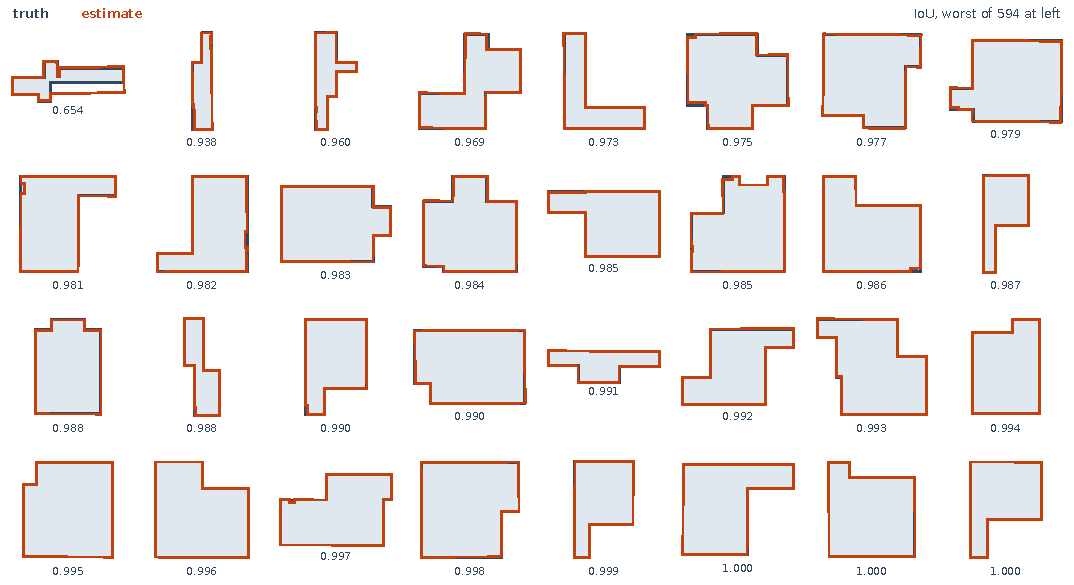
\includegraphics[width=\textwidth]{fig/mosaic}
\caption{\textbf{Thirty-two of the 594 annotated floor plans}, truth filled, estimate outlined, with
the achieved IoU beneath each. The panels are ordered by IoU and sampled evenly across \emph{every}
room that produced a closed polygon, so the population's worst room---IoU \num{0.654}---is the first
cell and the sample is not a selection of successes. The corpus's own shapes run from \num{6} to
\num{18} ground-truth corners, with the alcoves, wall columns and re-entrant corners that no
rectangle prior would admit.}
\label{fig:mosaic}
\end{figure*}

\emph{Does the epistemic term earn its place?} The explorer scores viewpoints by expected
information gain. To test whether that objective is what produces the accuracy above, we re-ran all
594 rooms with the epistemic term replaced by the frontier-and-coverage heuristic it superseded,
holding the estimator, the sensor model, the per-room seeds and the \num{900}-frame budget fixed.
\emph{We find no statistically detectable difference under this evaluation.} Paired over the 583
rooms both arms complete, the mean IoU
difference is \num{-0.0007} (95\% CI $[-0.0019, +0.0004]$, bootstrap over rooms), the heuristic
winning 263 rooms to 251; hard failures are 8 against 6; and the median frame at which the map first
becomes publishable differs by \num{6} frames (95\% CI $[-14, +28]$). Splitting by ground-truth
corner count recovers no difference in any band.

We report this because it bounds our own claim, and because the reason for the null is instructive.
Every room in this corpus ran to the frame cap in both arms: the room sizes are such that
\num{900} frames of any reasonable policy eventually sees every wall, so the \emph{final} map cannot
separate the policies, and an objective cannot be graded on an endpoint its own budget has saturated.
What the experiment supports is that the uncertainty is consumed---it gates publication, and the
explorer reads it. What it rules out is a claim we might otherwise have made: on rooms of this size,
the epistemic objective buys no measurable accuracy or speed over a simple heuristic. Whether it pays
under a tighter budget, or in the larger multi-room environments where a policy has room to waste
time, is not tested here.

\subsection{Is the reported uncertainty calibrated?}
\label{sec:calib}

For every room we take the final published polygon and match its corners one-to-one to the truth
corners by Hungarian assignment. Surplus corners on either side remain unmatched and are counted as
\emph{structure} errors---never as position error. This matters: nearest-vertex matching instead
yields a mean error of \SI{0.43}{\meter} against a median of \SI{0.023}{\meter}, because a spurious
corner has no truth counterpart and its ``error'' is meaningless.

Table~\ref{tab:calib} shows the effect of the systematic term of \eqref{eq:corner}. Without it, the
true error is flat at about \SI{2}{\centi\meter} across every band of declared $\sigma$: a corner
claiming \SI{1}{\centi\meter} is no more accurate than one claiming \SI{5}{\centi\meter}, and the
declared uncertainty ranks corners without predicting their error. The measured floor is
\SI{0.019}{\meter}, against a simulated sensor of \SI{0.020}{\meter} per return. Adding it as a
variance term---not a clamp---brings the declared $\sigma$ into agreement with the error that
occurs, at almost no cost in yield.

\begin{figure*}[t]
\centering
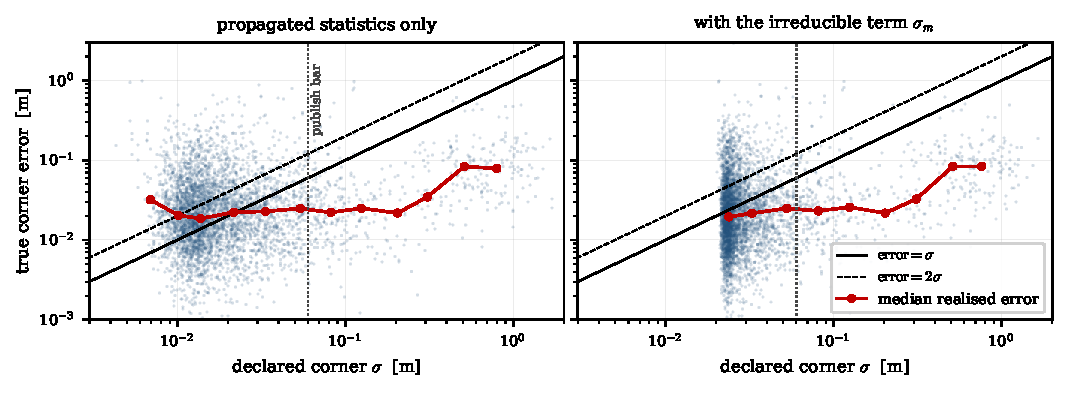
\includegraphics[width=\textwidth]{fig/calibration}
\caption{\textbf{Does the declared uncertainty track the realised error?} All \num{4344} matched
corners from the \num{586} annotated floor plans that produced a closed polygon: declared $\sigma$
against the error it actually made. \emph{Left}, propagating only the walls' statistical uncertainty:
the red median is flat, so a corner claiming \SI{1}{\centi\meter} is no more accurate than one
claiming \SI{5}{\centi\meter}, and the cloud sits far above $\mathrm{error}=\sigma$ at the tight end.
\emph{Right}, with the irreducible term of \eqref{eq:corner}: the median tracks the diagonal, so the
declared $\sigma$ is substantially more informative about the realised error and supports the
publication decision --- though, as the text reports, it remains weak as a fine-grained ranking. The
dotted line is the publication gate.}
\label{fig:calib}
\end{figure*}

\begin{table}[t]
\centering
% ── CAPTION SHORT, EXPLANATION IN A NOTE ────────────────────────────────────────────────────────
% IEEEtran sets TABLE captions in small caps. That is the house style and it suits a short title, but
% this caption was a nine-line paragraph, so the whole explanation rendered in small caps and read as
% shouting. The rule is structural, not cosmetic: a table caption gets a title, and anything the
% reader needs in order to interpret the numbers goes in a note below the rules, in normal type.
\caption{Calibration of the published corner $\sigma$}
\label{tab:calib}
% tabcolsep 6pt x 2 x 6 columns = 72pt of padding alone, which put this tabular 67.8pt OVER the
% column and let it run into the margin. Narrower padding plus \footnotesize fits it with room left.
\setlength{\tabcolsep}{2pt}
\footnotesize
\begin{tabular}{lccccc}
\toprule
& $\le 1\sigma$ & $\le 2\sigma$ & $\le 3\sigma$ & publish & holds \\
\midrule
no $\sigma_m$                & 46.7\% & 70.5\% & 81.2\% & 89.0\% & 85.8\% \\
$\sigma_m=\SI{2}{\centi\meter}$ & \textbf{65.3\%} & \textbf{85.0\%} & \textbf{91.2\%} & 89.0\% & 86.1\% \\
\emph{95\% CI, by room} & \scriptsize{[62.7, 67.9]} & \scriptsize{[83.2, 86.8]}
                             & \scriptsize{[89.9, 92.4]} & \scriptsize{[87.8, 90.4]}
                             & \scriptsize{[84.2, 87.8]} \\
\midrule
global $\sigma_c$ (fitted) & 65.3\% & --- & --- & 100\% & --- \\
\bottomrule
\end{tabular}

\vspace{2pt}
\begin{minipage}{\columnwidth}
\footnotesize
\num{4344} matched corners, from the \num{586} of \num{594} rooms that closed a polygon --- the other
\num{8} have no corners to match. \emph{publish} is the fraction passing the \SI{6}{\centi\meter}
gate, \emph{holds} the fraction whose claim is borne out. The first three columns are empirical
coverage, $P(\lVert e \rVert_2 \le k\sigma)$ --- \emph{not} a bound, since a standard deviation makes
no containment guarantee. Intervals are \num{2000}-sample bootstraps resampling \emph{rooms}, not
corners, which share a room's walls and trajectory. The last row is a deliberately favourable
baseline: one global $\sigma_c$ fitted \emph{post hoc} on this same corpus so its \num{1}$\sigma$
coverage matches ours exactly.
\end{minipage}
\end{table}

\emph{One global precision cannot do this job.} The last row of Table~\ref{tab:calib} is the
obvious alternative: a single $\sigma_c$ fitted to this very corpus, chosen so that it reproduces our
$1\sigma$ coverage exactly ($\sigma_c=\SI{0.0317}{\meter}$). It is therefore calibrated as favourably
as the data allow --- and it is still insufficient for the task. Being constant, it provides no
ranking of corners by realised error at all: a rank correlation is not merely zero but undefined,
since the predictor has no rank variation. Under the \SI{6}{\centi\meter} gate it publishes
\SI{100}{\percent} of corners, because every corner carries the same number and the gate has nothing
to separate. The post-hoc fit is not what defeats it: refitting $\sigma_c$ by \num{5}-fold
cross-validation over \emph{rooms} gives \SI{0.0318}{\meter} $\pm$ \SI{0.0002}{\meter} and a held-out
\num{1}$\sigma$ coverage of \SI{65.4}{\percent}, indistinguishable from the \SI{65.3}{\percent} it was
fitted to reach. The scalar is perfectly well calibrated \emph{on average} and generalises as such;
what it cannot do is vary. A scalar can be calibrated \emph{on average} and still be unable to tell one corner from
another, which is the distinction this paper is about.

\emph{What $\sigma$ is, and is not, good for.} Between the two gate classes the separation is clean
and survives the room-level interval: published corners have a median error of
\SI{0.0202}{\meter} (CI \SIrange{0.0185}{0.0220}{\meter}) against \SI{0.0364}{\meter}
(CI \SIrange{0.0312}{0.0446}{\meter}) for withheld ones, and the intervals do not overlap. Ranking
\emph{within} a class is weaker: the Spearman correlation between declared $\sigma$ and realised error
is \num{0.125} (CI \numrange{0.088}{0.161})--- significantly positive, but small. We report it
because it bounds the claim honestly: this $\sigma$ is a trustworthy \emph{decision variable} for the
publish/withhold question it is used for, not a fine-grained ordering of corners by accuracy.

\emph{The gate is a tolerance, not a tuned parameter.} The \SI{6}{\centi\meter} gate is the
downstream consumer's requirement---the clearance a planner in this stack needs a corner to be good
to---and was fixed before this evaluation rather than chosen on it. Nothing here turns on the value:
sweeping it, the median error of published corners is flat at \SIrange{1.99}{2.04}{\centi\meter} for
gates of \num{4}, \num{6}, \num{8} and \SI{10}{\centi\meter}, while the withheld median rises
monotonically from \SI{3.09}{\centi\meter} to \SI{5.33}{\centi\meter} and the published fraction from
\SI{81.1}{\percent} to \SI{93.2}{\percent}. The separation is therefore a property of the ordering,
not of where the cut is placed. Below \SI{2}{\centi\meter} the gate is vacuous in the other
direction: the smallest declared $\sigma$ in the corpus is \SI{0.0203}{\meter}, so a
\SI{2}{\centi\meter} gate publishes nothing.

\emph{The actionable claim.} Publication is gated at $\sigma \le \SI{6}{\centi\meter}$. A corner the
system declares publishable has a median true error of \SI{2.0}{\centi\meter} and lies within the
\SI{6}{\centi\meter} it claims in \SI{86.1}{\percent} of cases; a corner it withholds has a median
error of \SI{3.6}{\centi\meter} and meets the same criterion only \SI{63.7}{\percent} of the
time.
The gate discriminates, and the number it gates on now means something.

\subsection{The split on recorded depth}
\label{sec:real}

The decomposition in \eqref{eq:corner} claims that error separates into a part that averages away and
a part that does not. We measure both on MP3D-FPE~\cite{solarte2022dfpe}, which provides
real Matterport depth with camera trajectories and per-room annotated corners. Slicing the depth to a
horizontal band and fitting each annotated wall from the returns that land on it gives both terms
directly (588 segments, 120 rooms; the slice registers to the annotations with a median modal offset
of \SI{7.5}{\milli\meter}).

\begin{table}[t]
\centering
\caption{The two components, measured on real depth against annotated walls.}
\label{tab:real}
\setlength{\tabcolsep}{3pt}
\begin{tabular}{lSS}
\toprule
& {median (\si{\meter})} & {p90} \\
\midrule
scatter about the fitted wall (averages down) & 0.0149 & 0.0382 \\
fitted vs.\ annotated wall (does not) & 0.0181 & 0.0572 \\
\bottomrule
\end{tabular}
\end{table}

Two consequences. First, the simulated sensor model is consistent with, and slightly more
conservative than, the real-depth measurements: real depth scatters at \SI{1.5}{\centi\meter} against
the \SI{2.0}{\centi\meter} simulated, so the calibration above rests on a noise model that does not
flatter it. Second, the
systematic component is not explained by independent sensor noise alone: it survives at
\SI{1.8}{\centi\meter} in data whose per-return scatter is \SI{1.5}{\centi\meter}, and scatter that
averages down cannot produce an offset that does not. That is what sets up the next result.


\subsection{Closed-loop simulation with a LiDAR sensor model}
\label{sec:webots}

The experiments so far establish that the declared uncertainty is calibrated
(\S\ref{sec:calib}) and that its two components are real on real depth (\S\ref{sec:real}). Neither
shows the estimator \emph{using} them while it runs. This experiment does, on a robot driving a
simulated LiDAR in closed loop, in a room whose ground truth is exact.

The room is a rectangle of $\SI{6.000}{\meter} \times \SI{4.000}{\meter}$, taken from the wall solids of the world rather
than from any fitted model, with a \SI{1.06}{\meter} doorway in one wall. A rectangle is the useful
test here for a reason that is methodological rather than geometric: \emph{edge lengths and corner
angles are invariant to the map frame}, so the estimate can be scored with no rigid alignment. Every
other layout comparison in this literature must align first, and alignment absorbs the global pose
error into the score. Here it does not arise. We pre-registered the predictions before the run: the
polygon closes on four corners, the recovered width falls within two declared $\sigma$ of truth,
and---the outcome we were actually watching---if the pose channel's known defect, a covariance that
omits the repeatable part of the error (\S\ref{sec:notconstant}), extends to the layout channel, the
declared $\sigma$ will fall below the realised error while the robot is stationary and keep falling
the longer it sits.

It did not. Table~\ref{tab:webots} reports the run: \SI{665}{\second} parked, then a turn in place.

\begin{table}[t]
\centering
\caption{Closed loop, Webots, LiDAR sensor model. Ground truth is the world's wall solids;
$\sigma$ is the worst corner of the published polygon. The run is \SI{762}{\second} long; each column
is labelled with its time.}
\label{tab:webots}
\begin{tabular}{lccc}
\toprule
 & \SI{0}{\second} & \SI{665}{\second} & \SI{689}{\second} \\
\midrule
long edge   & \SI{5.994}{\meter} & \SI{5.995}{\meter} & \SI{5.994}{\meter} \\
short edge  & \SI{4.016}{\meter} & \SI{4.013}{\meter} & \SI{4.019}{\meter} \\
worst corner $\sigma$ & \SI{0.988}{\meter} & \SI{0.989}{\meter} & \textbf{\SI{0.048}{\meter}} \\
worst edge $\sigma_d$ & \SI{0.500}{\meter} & \SI{0.500}{\meter} & \SI{0.019}{\meter} \\
\bottomrule
\end{tabular}
\end{table}

\emph{The geometry was already accurate before the uncertainty became small.} Standing still, the
estimate was already
$\SI{5.994}{\meter} \times \SI{4.016}{\meter}$---within \SI{6}{\milli\meter} and \SI{16}{\milli\meter} of truth---while
the worst corner declared almost a metre of uncertainty and every edge offset sat at exactly its
\SI{0.500}{\meter} prior. Over \SI{665}{\second} and \num{13000} frames, with five wall segments
associating per frame, the worst corner $\sigma$ moved from \SI{0.9882}{\meter} to \SI{0.9885}{\meter} and
the edge prior did not move at all (four of \num{53284} logged edge values departed from
\SI{0.500}{\meter}). A turn in place, over the next \SI{24.5}{\second}, then dropped the worst corner
$\sigma$ by a factor of \num{21}, to \SI{0.048}{\meter}, while the geometry moved by millimetres. We
do not quote the size of that turn: this run logs the room model's pose, not the robot's, so the
rotation it performed is not recoverable from it. The third column is the \emph{first} frame the layout is publishable; $\sigma$
keeps falling afterwards, to \SI{0.031}{\meter} at \SI{719}{\second} and \SI{0.029}{\meter} at the
end of the run, but the log is sampled at
\SI{50}{\milli\second} only up to that frame and has a \SI{30}{\second} gap immediately after it, so
the turn is quoted to where it can be measured rather than to where it looks largest.

Two things this run cannot show. The map frame is \emph{gauge-free}---its origin and orientation are
wherever the estimator put them---and the log carries no ground-truth robot pose, so we report the
no heading error at all, which would describe our own gauge rather than the robot. For the same
reason both panels of Fig.~\ref{fig:teaser}
are drawn with the long axis horizontal: the re-anchor rotates the frame between them, and every
quantity claimed here---edge lengths, corner $\sigma$, the comparison with truth---is invariant to
that rotation.

This is the generative model's own arithmetic rather than a policy. A stationary robot observes the
same walls from the same viewpoint; the observations are not independent, so the information they
carry about the layout saturates. The estimator therefore cannot earn precision by waiting, and does
not claim any. Rotation changes the viewpoint, the observations stop repeating, and the precision
arrives at once. The final estimate is \SI{5.996}{\meter} and \SI{4.005}{\meter} against \SI{6.000}{\meter} and
\SI{4.000}{\meter}: errors of \SI{-4}{\milli\meter} and \SI{+5}{\milli\meter}, or \num{0.13} and \num{0.16} of
the $\sigma$ the system declared for them.

The same run shows the opposite behaviour in the pose channel, where correlated evidence does shrink
the covariance while the robot is parked. We report that as a measured defect in \S\ref{sec:limits}: it is the same
question asked of two channels, and only one of them answers it correctly, which is what makes the
comparison informative.

\subsection{Why a single global precision is insufficient}
\label{sec:notconstant}

In the same simulator, driving a \SI{166}{\meter} tour of a \num{20}-corner apartment, we log for
every corner candidate at the association gate the innovation and each term of its covariance:
\num{300007} candidates over \num{23551} frames, of which the association gate rejects
\SI{27}{\percent}. The tour length is measured from the logged trajectory rather than estimated. The reference layout here is traced from the building's floor plan rather
than read from the world, because that world's walls are meshes rather than parametrised solids; it
is therefore an imperfect map of a kind a deployed robot is often given, which is the point. Normalised innovation
squared ($\nis$, divided by its two degrees of freedom) equals 1 when a covariance matches the error
it claims.

Recovering inter-frame motion from the detections themselves---a rigid fit between consecutive
frames, so no pose log is needed---lets the population be split by what the robot is \emph{doing}.
Over \num{34} stationary stretches and \num{386} corner-stretch pairs, decomposing the innovation for
a fixed corner separates two parts cleanly: the part that \emph{repeats} has a median of
\SI{0.0574}{\meter} and the part that \emph{scatters} \SI{0.0066}{\meter}, a ratio of \num{8.7}, with
the bias exceeding the scatter in \SI{97}{\percent} of pairs. Averaging removes the second and cannot
touch the first.

\emph{The repeatable part is not a map error.} A map offset displaces the true corner, so the
detection re-expressed in the room frame must land in the same wrong place from every viewpoint. It
does not: across the \num{17} corners seen in three or more separate stretches, the spread
\emph{between} stretches is \SI{0.0442}{\meter} against \SI{0.0074}{\meter} \emph{within} one---a
factor of \num{6.0}, and of the same order as the bias itself. It is also not sensor noise, which is the part that
averages. It is a repeatable, viewpoint-dependent error that the model represents nowhere, and
standing still accumulates confidence against it from observations that carry no new information
about it.

\emph{The declared precision does not cover this.} Over the same stationary stretches the
pose-induced term $\sigma_{\text{pred}}$ has a median of \SI{0.046}{\meter} against a repeatable
innovation of \SI{0.057}{\meter}: the pose covariance carries no term the size of the bias. The
$\nis$ this produces depends on which population is asked, and we report both rather than choosing:
over every candidate it is \num{2.51} at rest and \num{2.28} in motion, and over the
\SI{73}{\percent} the association gate accepts, \num{0.75} and \num{0.80}. Neither sits at \num{1};
the total is too large before the gate and too small after it, and in both cases its pose term is
smaller than the bias it must cover.

\emph{How much of this is one run.} The magnitude is run-dependent, since each tour stops at
different viewpoints and that is exactly what a viewpoint-attached error predicts; the hardware run
below is a second point. What is stable is the shape, and that is what the argument uses.

\emph{The same measurement on a physical robot.} Everything above is simulated. We ran the same
pipeline and the same analysis script, unmodified, on a differential-drive robot carrying a
\num{3}-D LiDAR in an apartment-scale indoor space, localised against a layout obtained offline by a
SLAM system---the imperfect map of the kind argued for above---over \SI{295}{\meter} in three
sessions, with the estimator restarted between them (Table~\ref{tab:realtour}). Over \num{6}
stationary stretches and \num{46} corner-stretch pairs the repeating part has a median of
\SI{0.0624}{\meter} against \SI{0.0046}{\meter} that scatters, with the bias exceeding the scatter at
every stop and every corner but one; across the \num{10} corners seen from three or more stretches
the spread \emph{between} stretches is \SI{0.0459}{\meter} against \SI{0.0046}{\meter} \emph{within}
one, a factor of \num{9.9}. Over accepted candidates $\nis$ is \num{0.836}, against \num{0.782} in
simulation.

Both verdicts match the simulator's, and the replication is in the bias: \SI{0.0624}{\meter} against
\SI{0.0574}{\meter}, agreeing to \SI{5}{\milli\meter} on a different sensor and a different map. The
scattering part is smaller on hardware, in the direction \S\ref{sec:real} reports for a simulated
sensor deliberately set more conservative than real depth, so the ratio---\num{13.4} against
\num{8.7}---exceeds the simulated one for a reason that lives in its denominator rather than in the
systematic term the argument is about.

The real sample is much thinner than the simulated one---\num{46} pairs against \num{386}, six stops
against \num{34}---and we claim no more than agreement in shape. The protocol called for deliberate
stops at distinct places and orientations; the second session made none, and on the first session's
three stretches alone the between-stretch statistic read \num{1.6}, the opposite verdict. The third
session added three such stops, and nothing was collected after it. We report the sequence because it
is the statistic's own sensitivity: a viewpoint-attached error cannot be detected without viewpoint
diversity, and distance driven is no substitute for it.

\begin{table}[t]
\centering
\caption{The repeat/scatter split, simulated and on hardware}
\label{tab:realtour}
\setlength{\tabcolsep}{3pt}
\footnotesize
\begin{tabular}{lrrcccc}
\toprule
tour & stops & pairs & repeats & scatters & ratio & viewpoint \\
\midrule
simulated      & 34 & 386 & \SI{0.0574}{\meter} & \SI{0.0066}{\meter} & \num{8.7}$\times$ & \num{6.0}$\times$ (17) \\
physical robot & 6  & 46  & \SI{0.0624}{\meter} & \SI{0.0046}{\meter} & \num{13.4}$\times$ & \num{9.9}$\times$ (10) \\
\bottomrule
\end{tabular}

\vspace{2pt}
\begin{minipage}{\columnwidth}
\footnotesize
\emph{viewpoint} is the spread between stops divided by the spread within one, over the corners seen
at three or more stops (count in brackets); above \num{2} it rules out a fixed map offset.
\end{minipage}
\end{table}

A bias that repeats, follows the viewpoint and survives the move to hardware is the argument for
representing the offset as an inferred state
with a prior rather than a compiled-in number.

\subsection{Calibration as a diagnostic}

Requiring precisions to mean what they say found three defects of one kind---uncertainty that
averages down past an error that does not, in three distinct places. In the \emph{layout} corner
$\sigma$ of Table~\ref{tab:calib} the systematic term was absent. In the \emph{corner detector's}
covariance it was present twice under two names for one quantity, making that channel
\num{2.1}$\times$ too timid; removing the duplicate and measuring the survivor moved $\nis$ from
\num{0.47} to \num{1.03} over accepted candidates on the tour it was measured on. In the \emph{pose}
covariance feeding $\sigma_{\text{pred}}$ it is absent again,
and was found by an instrument pointed at the layout. We regard the third as the strongest evidence that the formulation
does work rather than description: nothing in a pipeline of separately-tuned heuristics depends on a
precision being right, so nothing in it would have flagged any of the three.

\section{Limitations}
\label{sec:limits}

Observations in \S\ref{sec:geom} and \S\ref{sec:calib} are simulated from the annotated polygons;
\S\ref{sec:real} validates the noise model but not the full pipeline on recorded data, and the
hardware run of \S\ref{sec:notconstant} measures one channel rather than closing the loop. Layout
accuracy has not been measured on a physical robot, and doing so needs a surveyed reference we do not
have. We attempted a full pipeline evaluation on
MP3D-FPE~\cite{solarte2022dfpe} and report a negative result we believe is useful to others. Because
it annotates \emph{rooms inside open-plan buildings} while a \SI{360}{\degree} depth sensor sees
through every doorway, a median \SI{57}{\percent} of returns fall outside the room being scored
(\num{0} of its \num{401} rooms fall below \SI{10}{\percent}); taking the union of a floor's rooms
still leaves \SI{50}{\percent} outside, because corridors and stairwells are unannotated. No
granularity makes the annotation and the observation describe the same region, so this corpus---and,
we expect, any room-annotated building corpus---cannot grade a method that models a \emph{bounded}
room. The \num{0.14} IoU the corpus yields under these conditions measures that
mismatch rather than the estimator, and we report the mismatch instead.
Finally, the pose-covariance defect of \S\ref{sec:notconstant} is measured but not fixed; the cure we
argue for---a per-wall offset state with the measured prior---is future work.

\section{Conclusion}

A layout estimate that a robot can act on needs an uncertainty a robot can check. We have shown that
such an uncertainty can be maintained online, that it can be validated against ground truth at scale,
and that it becomes useful once something downstream depends on it. Requiring precisions to be
calibrated was not bookkeeping: it exposed three defects, and it showed that a quantity commonly
treated as a constant is not one.

\section*{Acknowledgements}

% ── DOUBLE-ANONYMOUS: NOTHING HERE MAY IDENTIFY THE AUTHORS ────────────────────────────────────────
% Funding bodies, grant numbers, institutions and colleagues by name go in at CAMERA-READY, not now —
% they are the usual way an acknowledgements section breaks a blind review. The AI disclosure below
% does NOT identify anyone and IEEE requires it to be here, so it stays in the anonymous submission.
\ifcameraready
This work was co-funded by the FEDER Project 0124\_EUROAGE\_MAS\_4\_E under the POCTEP Programme
2021--2027, and by the R\&D\&i project PID2022-137344OB-C31, supported by
MICIU/AEI/10.13039/501100011033 and ``FEDER, Una manera de hacer Europa''. Additional co-funding was
provided by the European Union through the European Regional Development Fund (85\%) and by the Junta
de Extremadura (Grant GR24194). The managing authority is the Ministerio de Hacienda (Spain). This
work was also supported by the SWEET Project, a Horizon Europe Marie Sk\l{}odowska-Curie action
(Agreement No.\ 101168792).
\fi

The authors used a large language model (Anthropic's Claude) as a writing and analysis assistant. Its
contributions were: generating the figures from the authors' own experimental data, by scripts that
are part of the submitted artefact; performing the bootstrap analysis of
Table~\ref{tab:calib}; drafting \S\ref{sec:webots}; and copy-editing throughout. Every number reported
in this paper was produced by the authors' own experiments and was checked against the recorded run
data; the model generated no data and performed no experiment. The authors take full responsibility
for the content, including all claims and their supporting evidence.

\balance
\bibliographystyle{IEEEtran}
\bibliography{refs}

\end{document}
